\documentclass{article}
\usepackage{graphicx}

\usepackage[utf8]{inputenc}

\title{Aplicação TPC-W altamente disponível}
\author{Grupo 3}
\date{March 2016}

\graphicspath{ {images/} }
\begin{document}

\maketitle

\section{Gerando a aplicação Web}
O primeiro passo foi gerar a aplicação web a ser estudada.

Para isso, utilizamos os seguintes aplicativos.


Banco de dados PostgreSQL
    
Servidor web Tomcat
    
Web Benchmark TPC-W
    
Emulador de navegadores RBE

Gnuplot, para gerar gráficos.


\section{Transferir arquivos remotamente}

scp -r ra082674@cbn3.lab.ic.unicamp.br:/nfs/wiki .
// scp origem destino

->OBS:  Editor de Latex Online
https://pt.sharelatex.com
Usuário: rodrigo.ssilva@gmail.com
Senha: mc4372016

->OBS: como dar append do conteúdo de um arquivo para outro
http://www.tecmint.com/13-basic-cat-command-examples-in-linux/
cat file_origem>>file_destino

OBS:->  como copiar colar no VIM
http://vim.wikia.com/wiki/Copy,_cut_and_paste

OBS: atualizar varivael de ambiente PATH
export PATH=${JAVA_HOME}/bin

------------------------------------------------------------------------------------
→ configurando SSH 
(supondo que já se encontra conectado na rede do IC)
SSH:


Entrar na pasta ~/.ssh no computador da onde voce vai executar ssh, editar arquivo config
Host ncbn3
HostName cbn3.lab.ic.unicamp.br
User raXXXYYY

onde XXXYYY é o numero de RA de cada aluno

Geração de Chaves:

Todos devem gerar um par de chaves pública e privada para permitir o acesso a maquina cbn3 do cluster sem usar senhas.

Para isso, deve-se abrir o terminal na sua máquina e executar os seguintes comandos:

$ ssh-keygen -t rsa


Esse comando gera as chaves pública (id_rsa.pub) e privada (id_rsa) e as salva na pasta .ssh/

Ele vai pedir um nome de arquivo e uma senha/confirmação de senha. Pode deixar todos em branco.

Em seguida rode o seguinte comando
$ ssh-copy-id cbn3

Ele vai te pedir a sua senha para logar na maquina cbn3 do cluster, onde voce poe a sua senha de login no computador da rede do IC.
Esse comando vai copiar a chave publica para o arquivo authorized_keys na pasta .ssh do seu usuário da dasha.


A partir de agora você deve conseguir logar na cbn3 sem ter que colocar a senha apenas digitando o seguinte comando no terminal:
$ ssh cbn3


→ configurando GIT 

instale o git grupo03.git na home do lider

crie o diretorio grupo03 na home

primeiro da clone na pasta do lider (ra082674……)

depois da um pull pra atualizar

depois pra adicionar algum arquivo na pasta do lider

da add

obs: se vc dar git status, aparece os arquivos novos a serem pushados

depois commit -m

depois push



→ configurando PostgreSQL 


-> tirado de http://www.ggte.unicamp.br/eam/mod/wiki/view.php?id=17445
Configurado Tomcat
-> configurar Tomcat

criar PATH para a pasta do Tomcat onde está instalado tpcw:

/var/lib/tomcat7/webapps/tpcw




para reiniciar o Tomcat:
$ invoke-rc.d tomcat7 restart

entrando em ssh3.lab.ic.unicamp.br:8080, verá ele funcionando
segundo o prof, isso aki tem que dar deploy no TPCW para aparecer ele no ar:
http://cbn3.lab.ic.unicamp.br:8080/

Seguido conforme tutorial “tirado”

Instalaram o postgresql 9.5

# pg_dropcluster --stop 9.5 main
# pg_createcluster 9.5 main -u [user_name]

nova senha para usuário postgres (usuário responsável pelo DB): postgres

adduser tpcw-user
adduser buzato

para acessar o usuario postgres:
$ su -s /bin/bash postgres

senha: postgres

como usuario postgres, rodar o banco de dados do dump q eh do tpcw:
$ psql tpcw

lista todos 
$psql -l

para fechar postgres:
posgres#	\q

para sair do usuario postgres e retornar ao usuario ra….. no cbn3:
$	exit

para sair de qualquer menu do postgres# basta teclar 
# q


TPCW:

http://cbn3.lab.ic.unicamp.br:8080/tpcw/TPCW_home_interaction

adicionamos nossos usuários no grupo tomcat7 para termos permissões para criar a aplicação na pasta /var/lib/tomcat7

criamos a Pasta tpcw, e dentro dela mais dua pastas, Images e WEB-INF.
copiamos as images de  /nfs  para Images e em na pasta classes compilamos os arquivos .java mantendo os .classes nesta pasta

mudamos as permissões e reiniciamos o servidor
$ chgrp tomcat7 . -R
$ chmod o-rwx . -R
# invoke-rc.d tomcat7 restart
Integrando com PostGreSQL

baixou o jar de um site
deu scp do .jar para a pasta grupo03 na rede cbn3
colocou esse .jar na path certa dentro da pasta tomcat7

--------->  




RBE:

executando o comando:
$ java -cp /nfs/rbe/rbe.jar rbe.RBE -EB rbe.EBTPCW1Factory 1 -CUST 10 -ITEM 1000 -OUT out.debug.m -WWW http://cbn3.lab.ic.unicamp.br:8080/tpcw/ -RU 10 -MI 120 -RD 10 -DEBUG 10




**** DEVE-SE APAGAR O ARQUIVO DE SAÍDA out.debug.m na pasta do tpcw do tomcat antes de se executar RBE de novo


Depois de um certo tempo, teremos o arquivo out.m, mas para analizá-lo, precisamos utilizar o programa que o professor disponibilizou, para isso: 
$ python /nfs/rbe/analyze.py out.debug.m
OBS: Lembrando que esse comando deve ser dado apenas depois de ter seguido as instruções do log "Configurando path para acesso aos scripts" sobre exportar a path /srv/ do nosso grupo no arquivo .bashrc
Pronto, já temos o arquivo .plot e alguns dados que o analize gera, mas para poder ver os gráficos, faça o seguinte:
Rode o comando e copie a saída: cat tpcw-run.plot
Agora abra o gnuplot, para fazer isso rode: gnuplot
Dentro do gnuplot, rode o seguinte comando: set terminal dumb
OBS: Essa é uma forma bem simples de ver os gráficos
Pronto, tudo está configurado. Agora cole o que a saída da instrução 6.1. ainda dentro do gnuplot. Será algo parecido com isso:
plot "tpcw-run.histogram" using 1:2 title "WIPS" with lines
Para voltar ao terminal e sair do gnuplot digite: quit





http://www.ggte.unicamp.br/eam/mod/wiki/view.php?pageid=154



Fizemos o que está aqui E GoogleDocs
http://www.ggte.unicamp.br/eam/mod/wiki/view.php?pageid=145
usuário é postgres/postgres

https://tomcat.apache.org/tomcat-7.0-doc/jdbc-pool.html baixamos o 41

copiamos de http://www.ggte.unicamp.br/eam/pluginfile.php/188108/mod_wiki/attachments/132/tomcat7-context.xml e colocamos tudo isso no Context


copiamos de http://www.ggte.unicamp.br/eam/pluginfile.php/188108/mod_wiki/attachments/132/tomcat7-server.xml e colocamos em  GlobalNamingResources

usuário e senha é postgres

"Reinicie o Tomcat e verifique se há erros no arquivo $CATALINA_BASE/log/catalina.out"
verificamos esse log para ver os erros que estavam acontecendo
como usuario e senha invalido
hostname invalido.


após cada alteração, demos invoke-rc.d tomcat7 restart

\section{Resultados medidos}

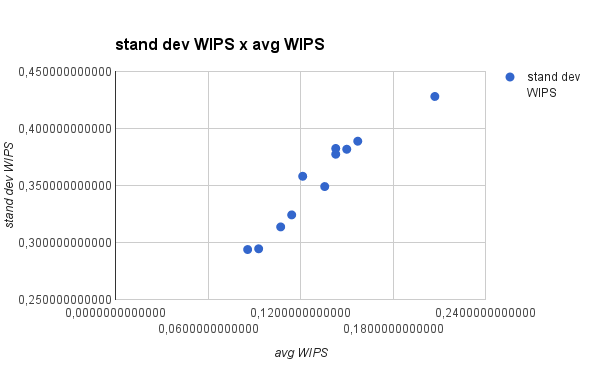
\includegraphics{image}
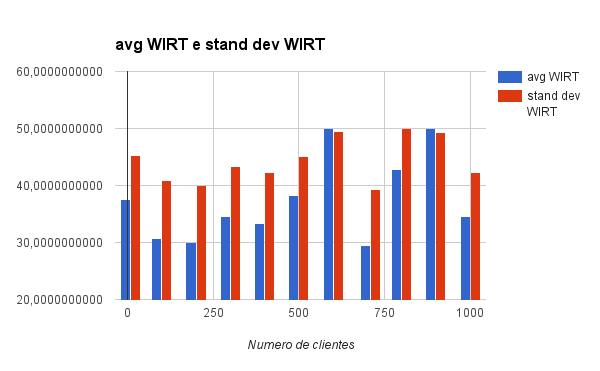
\includegraphics{imageb}



\end{document}
